\documentclass[12pt,a4paper]{article}

% Compile with XeLaTeX or LuaLaTeX.
\usepackage{fontspec}
\usepackage{polyglossia}
\setdefaultlanguage{russian}
\setmainfont{Liberation Serif}
\setmonofont{Liberation Mono}
\usepackage{amsmath,amssymb}
\usepackage{geometry}
\geometry{left=2.5cm,right=2cm,top=2cm,bottom=2cm}
\usepackage{graphicx}
\usepackage{float}
\usepackage{booktabs}
\usepackage{longtable}
\usepackage{array}
\usepackage{caption}
\usepackage{hyperref}
\hypersetup{colorlinks=true,linkcolor=black,urlcolor=blue,citecolor=black}
\usepackage{microtype}
\setlength{\parindent}{1.25cm}
\setlength{\parskip}{3pt}
\setlength{\emergencystretch}{3em}
\renewcommand{\arraystretch}{1.2}

\title{\textbf{Проверка гипотезы H1: гарантированный выбор модели при неизвестных исходах}}
\author{}
\date{25 октября 2026 г.}

\begin{document}
\maketitle

\begin{center}
\textit{Итоговый отчёт по реализации C0--C3 и контролируемым экспериментам на подготовленной тестовой выборке RLMS}
\end{center}

\noindent\textbf{Объём исследования:} подготовленная тестовая выборка RLMS; международные панели в текущий объём не входят.

\section*{Аннотация}
Исследуется гипотеза H1: в некоторых практически релевантных ситуациях можно выбрать модель, чьё качество гарантированно не хуже качества лучшей модели из фиксированного набора более чем на заданный допуск $\varepsilon$, даже если часть бинарных целевых меток неизвестна.

Реализованы четыре подхода: C0 --- отдельные интервалы ошибок; C1 --- точные парные интервалы; C2 --- интервалы с дополнительным ограничением на число положительных исходов; C3 --- статистические границы после случайного аудита. Реализация проверена автоматическими тестами, а поведение методов исследовано на синтетических примерах и на подготовленной тестовой когорте, относимой к RLMS-HSE, с искусственным сокрытием меток.

В тестовой когорте 49\,651 наблюдение и 15\,917 уникальных людей. В контролируемых построчных и человеко-уровневых экспериментах C1 давал существенно более узкие границы, чем C0. Дополнительный эксперимент изучал C2 и C3 при заранее заданных бюджетах случайного аудита. Результаты относятся к одной подготовленной тестовой когорте и искусственным механизмам сокрытия; они не устанавливают механизм естественных пропусков и не доказывают универсальную переносимость на другие выборки.

\section{Постановка задачи}
Пусть имеется $N$ наблюдений и $K$ заранее зафиксированных моделей. Прогноз модели $k$ для наблюдения $i$ обозначается $p_{ik}$, бинарная целевая метка --- $y_i\in\{0,1\}$. Множество наблюдений с известными метками обозначается $O$, множество скрытых меток --- $M$. В базовой постановке используются одинаковые веса $w_i=1/N$; в общем случае веса неотрицательны и суммируются к единице.

Полный риск модели определяется как
\[
R_k=\sum_i w_i(p_{ik}-y_i)^2.
\]
Истинный regret равен
\[
\operatorname{true\_regret}_k=R_k-\min_j R_j
\]
и измеряет разницу с лучшей моделью внутри рассматриваемого набора. Это сравнительная, а не абсолютная гарантия: даже сертифицированная модель может иметь неудовлетворительное абсолютное качество.

Для каждой пары моделей вычисляются нижняя и верхняя границы $L_{kj}$ и $U_{kj}$ возможной разности рисков $R_k-R_j$ при всех допустимых заполнениях скрытых меток. Затем
\[
G_k=\max_j U_{kj}.
\]
Выбирается кандидат с минимальным $G_k$; если $G_k\leq\varepsilon$, результат помечается \texttt{certified}. В противном случае возвращается \texttt{insufficient\_evidence}. При несовместимости дополнительных ограничений должен возвращаться статус \texttt{assumption\_infeasible}.

\section{Рассматриваемые методы}
\subsection{C0 --- отдельные интервалы}
Для каждой модели отдельно рассчитываются нижняя и верхняя возможные ошибки, после чего парные границы получают вычитанием этих экстремумов. Метод корректен, но консервативен: худшие случаи для двух моделей могут быть несовместимы.

\subsection{C1 --- точные парные интервалы}
Разность квадратов потерь двух моделей представляется как $a_i+b_i y_i$. Для известных меток вклады фиксированы; для скрытой бинарной метки минимум и максимум выбираются из двух допустимых значений. При независимой допустимости скрытых меток полученные парные границы точны для заданной постановки. Дополнительные предположения о механизме пропусков не требуются.

\subsection{C2 --- ограничения на количество единиц}
Для заранее заданной группы скрытых наблюдений предполагается, что число положительных исходов находится в интервале $[A_g,B_g]$. Это дополнительная информация, а не бесплатное знание. Границы рассчитываются сортировкой коэффициентов и перебором допустимого числа единиц. Если ограничение построено по аудиту, оно является вероятностным и должно интерпретироваться соответственно. Неверное ограничение может привести к ложному сертификату.

\subsection{C3 --- статистический аудит}
Из скрытой части случайно, без возвращения, раскрывается заранее заданное число меток. Для парных разностей рассчитывается статистическая оценка и радиус Hoeffding-типа [1]; статистические интервалы пересекаются с границами C1. Если пересечение пусто, статистическое событие считается неуспешным и метод возвращается к C1. Гарантия условна относительно корректного случайного дизайна и заранее перечисленных бюджетов аудита.

\section{Данные и протокол экспериментов}
Использована подготовленная тестовая таблица проекта Task 2, относимая к RLMS-HSE. Она содержит 49\,651 строку и 15\,917 уникальных идентификаторов людей. В таблице доступны бинарные целевые метки и прогнозы трёх фиксированных моделей: Transition baseline, Logistic Regression и HistGradientBoosting. В рамках данного отчёта происхождение каждой записи независимо по исходным файлам RLMS не верифицировалось; поэтому далее используется формулировка «подготовленная тестовая выборка RLMS».

На полной тестовой когорте рассчитаны Brier scores. Затем метки искусственно скрывались либо независимо на уровне строк, либо целиком для выбранных людей. Для каждого сценария использовалось 30 масок при долях пропусков 10\%, 20\% и 40\%. Поскольку в контролируемом эксперименте исходные метки известны исследователю, истинный regret можно проверить относительно полной когорты.

Для дополнительного аудита исходно скрытой части заранее задавались бюджеты 10\%, 25\%, 50\% и 75\% от числа скрытых меток. Для C2 использовалась поправка на четыре заранее заданных бюджета через $\alpha/4$; для C3 задавалось число бюджетов $n_{\text{budgets}}=4$. Это контролируемый эксперимент с искусственным сокрытием и случайным раскрытием, а не исследование естественного механизма отсутствия меток.

\section{Проверка реализации}
Автоматический набор тестов завершился результатом \texttt{27 passed}. В проекте присутствуют тесты точного перебора C1, инвариантов парных границ, диагональных элементов, ширины интервала, обновления границ после раскрытия метки, дублирования кандидата, скрытых меток и граничных случаев.

В исходном синтетическом аудите C1 сравнивался с полным перебором допустимых заполнений: для 288 случаев максимальное расхождение было порядка $3\cdot10^{-16}$. Отдельный синтетический аудит C3 содержит 96 конфигураций по 2\,000 повторений, всего 192\,000 повторений; в сохранённых прогонах статистических нарушений не зарегистрировано. Это эмпирическая проверка реализации, а не замена математического обоснования.

В синтетическом стресс-тесте C2 при намеренно нарушенных ограничениях зафиксировано 1\,011 ложных сертификатов из 17\,256 выданных сертификатов в совокупности по всем рассмотренным прогонам. В сохранённой сводке максимальная доля ложных сертификатов среди выданных в отдельной конфигурации составляет около 25,9\% (590 из 2\,276 сертификатов). Это ожидаемо: гарантия C2 действует только при корректности дополнительного ограничения.

\section{Качество фиксированных прогнозных моделей}
На полной подготовленной тестовой когорте получены следующие значения Brier score:

\begin{table}[H]
\centering
\begin{tabular}{lr}
\toprule
Модель & Brier score\\
\midrule
Transition baseline & 0,063989\\
Logistic Regression & 0,060968\\
HistGradientBoosting & 0,057416\\
\bottomrule
\end{tabular}
\caption{Качество прогнозных моделей на тестовой когорте}
\end{table}

По Brier score лучший результат показала HistGradientBoosting. Этот результат характеризует качество прогнозов на данной тестовой выборке, но сам по себе не является гарантией выбора при неизвестных исходах.

\section{Результаты C0 и C1 при искусственном сокрытии строк}
Среднее значение $G$ по 30 маскам для каждой доли пропусков показывает преимущество C1 по ширине гарантированной верхней границы regret. Истинный regret в обновлённых результатах рассчитывался относительно полной исходной когорты, а не только оставшихся наблюдаемых строк.

\begin{table}[H]
\centering
\begin{tabular}{rrr}
\toprule
Доля скрытых строк & C0: среднее $G$ & C1: среднее $G$\\
\midrule
10\% & 0,078668 & 0,003153\\
20\% & 0,159635 & 0,010504\\
40\% & 0,318038 & 0,018502\\
\bottomrule
\end{tabular}
\caption{Среднее значение верхней границы regret при сокрытии отдельных строк}
\end{table}

\begin{figure}[H]
\centering
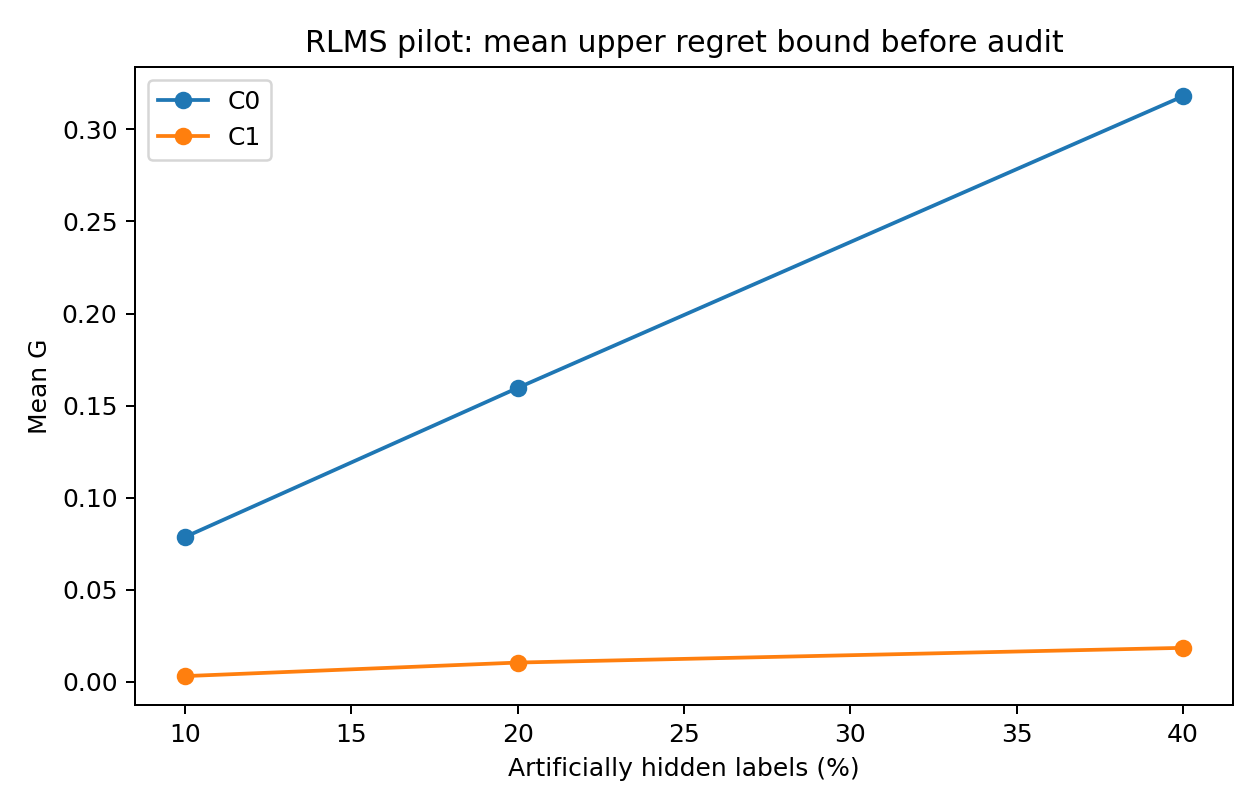
\includegraphics[width=0.85\textwidth]{figures/rlms_mean_G_C0_C1.png}
\caption{Среднее $G$ для C0 и C1 при разных долях скрытых меток}
\end{figure}

\section{Сокрытие целых людей}
Дополнительно скрывались метки всех наблюдений случайно выбранных людей, чтобы учесть повторные годовые записи одного идентификатора. Использовалось 30 повторений на каждую долю скрытых людей.

\begin{table}[H]
\centering
\begin{tabular}{rrr}
\toprule
Доля скрытых людей & C0: среднее $G$ & C1: среднее $G$\\
\midrule
10\% & 0,078166 & 0,003137\\
20\% & 0,159547 & 0,010482\\
40\% & 0,317886 & 0,018461\\
\bottomrule
\end{tabular}
\caption{Среднее значение верхней границы regret при сокрытии целых людей}
\end{table}

\begin{table}[H]
\centering
\begin{tabular}{rrr}
\toprule
Доля скрытых людей & $\varepsilon$ & Частота сертификации C1\\
\midrule
10\% & 0,0025 & 0\%\\
10\% & 0,005 & 100\%\\
20\% & 0,01 & 3,3\%\\
20\% & 0,02 & 100\%\\
40\% & 0,01 & 0\%\\
40\% & 0,02 & 100\%\\
\bottomrule
\end{tabular}
\caption{Примеры частоты сертификации C1 при разных $\varepsilon$}
\end{table}

\section{Дополнительный аудит C2/C3}
Для каждой исходной доли скрытых меток и каждого бюджета аудита сравнивались C0/C1 после тех же раскрытий, C2 с аудиторным ограничением на количество единиц и C3 со статистическими границами. В таблице ниже приведены частоты сертификации при $\varepsilon=0,01$. Частоты рассчитаны по 30 маскам на комбинацию условий.

\begin{table}[H]
\centering
\begin{tabular}{rrrrr}
\toprule
Исходно скрыто & Бюджет аудита & C1 & C2 & C3\\
\midrule
20\% & 10\% & 90\% & 100\% & 90\%\\
20\% & 25\% & 100\% & 100\% & 100\%\\
20\% & 50\% & 100\% & 100\% & 100\%\\
20\% & 75\% & 100\% & 100\% & 100\%\\
40\% & 10\% & 0\% & 0\% & 0\%\\
40\% & 25\% & 0\% & 0\% & 0\%\\
40\% & 50\% & 0\% & 0\% & 100\%\\
40\% & 75\% & 100\% & 100\% & 100\%\\
\bottomrule
\end{tabular}
\caption{Частота сертификации при $\varepsilon=0,01$ и различных бюджетах аудита}
\end{table}

\noindent\textit{Примечание.} Бюджет аудита выражен как доля от исходно скрытых меток. Частоты рассчитаны по 30 маскам для каждой комбинации условий. Все значения сверены с исходной сводной таблицей эксперимента.

\begin{figure}[H]
\centering
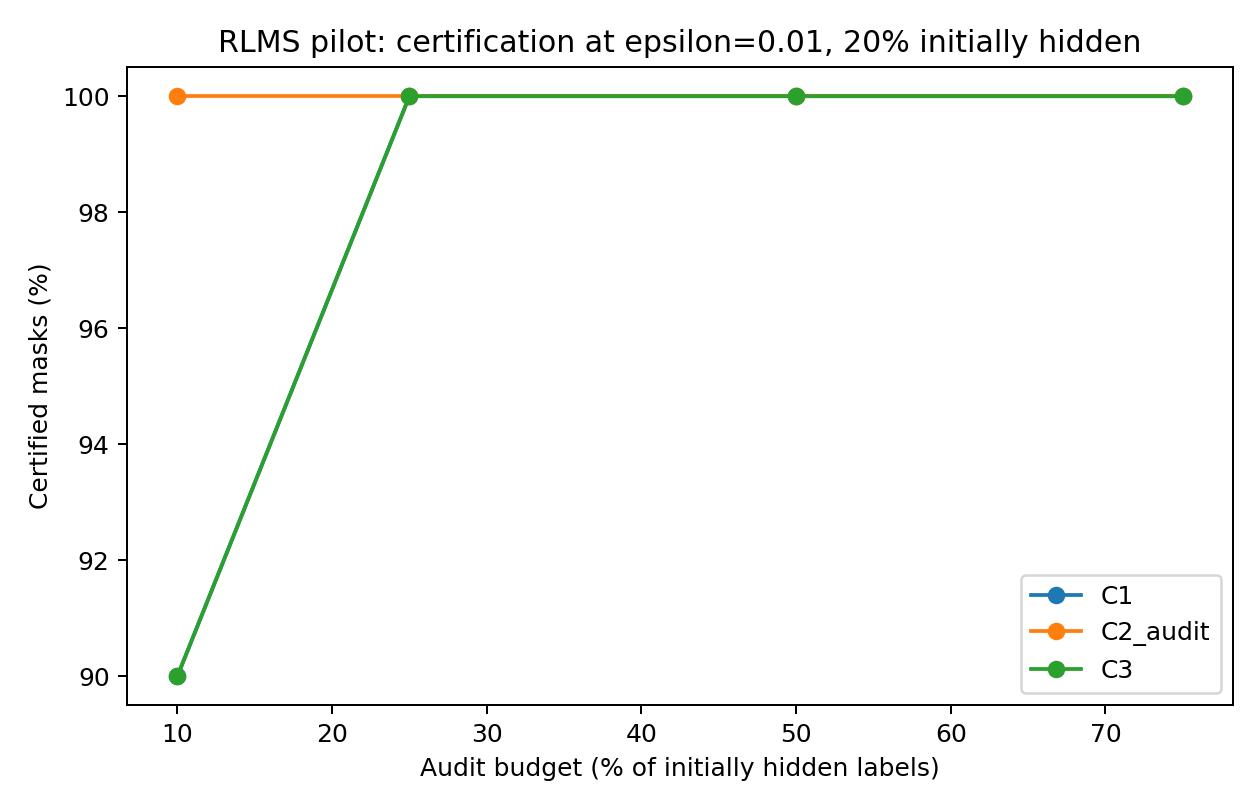
\includegraphics[width=0.85\textwidth]{figures/rlms_audit_certification_missing_20.png}
\caption{Частота сертификации при 20\% исходно скрытых меток}
\end{figure}

\begin{figure}[H]
\centering
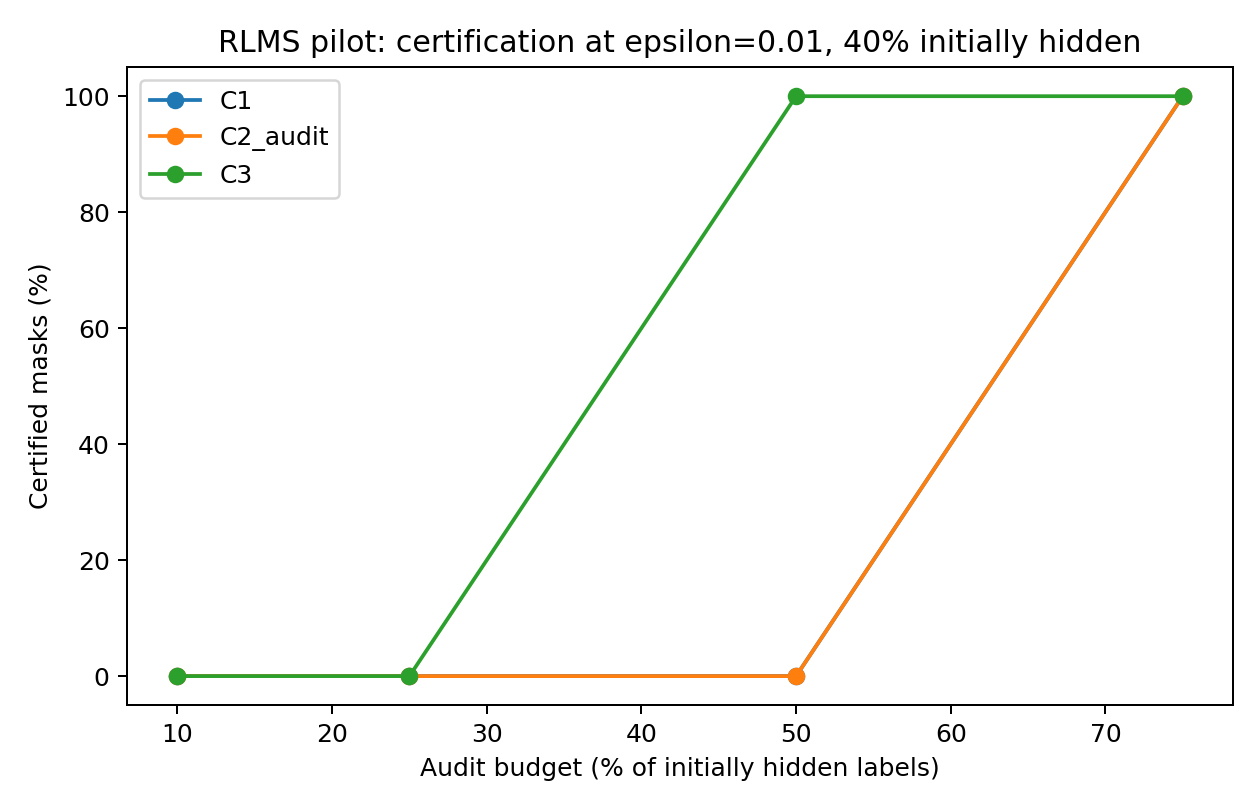
\includegraphics[width=0.85\textwidth]{figures/rlms_audit_certification_missing_40.png}
\caption{Частота сертификации при 40\% исходно скрытых меток}
\end{figure}

\section{Сравнение с point-estimate baseline}
\sloppy
На тех же 90 построчных масках выполнены complete-case, model-assisted plug-in и IPW с известной вероятностью включения, соответствующей искусственному MCAR-сокрытию. Вспомогательная логистическая модель для plug-in обучалась только на train-периоде с признаками возраста, пола и образования.

\begin{table}[H]
\centering
\begin{tabular}{llll}
\toprule
Доля пропусков & Complete-case & Model-assisted plug-in & IPW\\
\midrule
10\% & HGB (30/30) & HGB (30/30) & HGB (30/30)\\
20\% & HGB (30/30) & HGB (30/30) & HGB (30/30)\\
40\% & HGB (30/30) & Logistic Regression (30/30) & HGB (30/30)\\
\bottomrule
\end{tabular}
\caption{Выбор модели point-estimate baseline на искусственных масках}
\end{table}

При 10\% и 20\% пропусков все три baseline во всех 30 масках выбирали HistGradientBoosting (далее HGB), которая была лучшей по полной тестовой когорте.

При 40\% пропусков complete-case и IPW выбирали HistGradientBoosting во всех масках. Model-assisted выбирал Logistic Regression, полный true regret которой составлял 0,003552. Эти методы выдают рекомендации, но не сертификаты.

\fussy
\section{Ограничения}
\begin{enumerate}
\item Искусственное сокрытие меток не доказывает, что естественные пропуски в исходных данных возникают по тому же механизму. Эксперименты не устанавливают, являются ли реальные пропуски MCAR, MAR или MNAR.
\item Эмпирические выводы относятся к одной подготовленной тестовой когорте и трём фиксированным моделям. Они не доказывают универсальную переносимость на другие выборки, периоды или модели.
\item C1 сертифицирует близость к лучшей модели внутри заданного набора, а не абсолютную точность прогнозирования.
\item C2 зависит от корректности ограничений на число единиц. Если предпосылка неверна и противоречие ещё не выявлено, сертификат может оказаться ложным.
\item C3 даёт вероятностную гарантию только при соблюдении случайного дизайна аудита, равных весов и заранее заданных бюджетов. Адаптивная проверка после каждого нового размера выборки требует отдельного обоснования.
\item Проверки на NLSY97, UKHLS и PSID отложены и не входят в текущий объём работы.
\end{enumerate}

\section{Заключение}
В рамках выбранного объёма RLMS реализованы и проверены C0--C3, проведены синтетические проверки, контролируемые эксперименты с искусственными пропусками на уровне строк и людей, сравнение с point-estimate baseline, а также дополнительный аудит C2/C3 при заранее заданных бюджетах. Автоматические тесты прошли: 27 passed.

Главный эмпирический результат состоит в том, что на рассмотренной тестовой когорте C1 даёт существенно более узкие границы $G$, чем C0, при сокрытии отдельных строк и целых людей. Дополнительный аудит в отдельных режимах повышает частоту сертификации; величина эффекта зависит от доли пропусков, бюджета аудита и $\varepsilon$.

Итоговая формулировка H1: в рассмотренных контролируемых сценариях можно сертифицировать модель с regret не выше $\varepsilon$, даже если часть бинарных исходов скрыта, когда рассчитанная граница $G$ не превышает $\varepsilon$. Это подтверждает реализуемость конкретных правил выбора в заданной постановке, но не означает, что сертификат будет доступен при любой доле пропусков или что результаты автоматически переносятся на естественные пропуски и другие наборы данных.

\section*{Список литературы}
\begin{enumerate}
\item Hoeffding, W. Probability Inequalities for Sums of Bounded Random Variables. \textit{Journal of the American Statistical Association}, 1963. DOI: \href{https://doi.org/10.1080/01621459.1963.10500830}{10.1080/01621459.1963.10500830}. Используется как стандартное основание для статистической границы C3; собственный новый теоретический результат в этой работе не заявляется.
\end{enumerate}

\section*{Приложение. Воспроизводимость}
\sloppy
В комплекте проекта сохранены исходный код, настройки, автоматические тесты, входная таблица эксперимента и построчные результаты. Международные панели NLSY97, UKHLS и PSID намеренно не включены в текущий объём. Происхождение подготовленной тестовой таблицы из исходных файлов RLMS отдельно не верифицировалось; поэтому эмпирические результаты следует трактовать как результаты на подготовленной выборке, обозначенной в проекте как RLMS.

\end{document}
